\subsection{Zufallsvariable}
$P[X = x] = 0$
für stetige Zufallsvariablen ist die Wahrscheinlichkeit einer einzigen Variable gleich 0\\
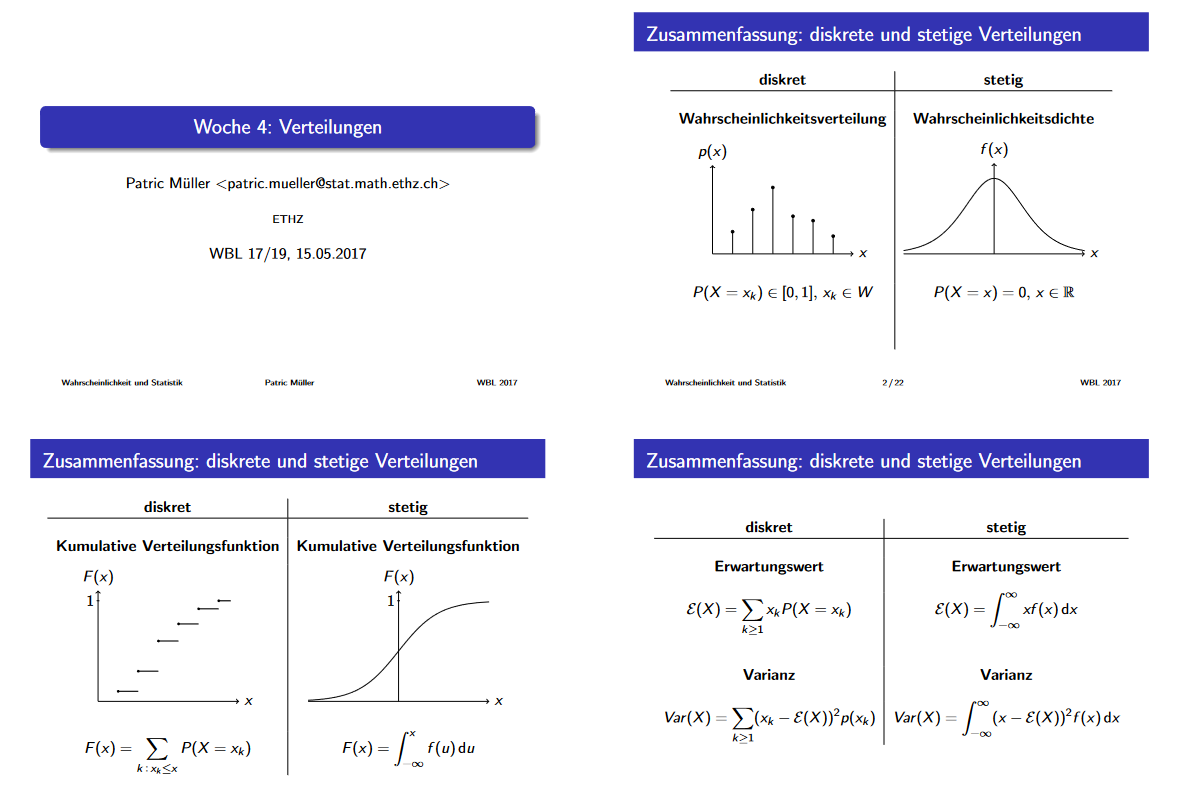
\includegraphics[width=\columnwidth]{diskrete_stetige_verteilung.png}\\
Sein $ (\Omega, \F, P)$ ein Wahrscheinlichkeitsraum. Also $\Omega$ ein
Grundraum, $\F \subseteq 2^\Omega$ die beobachtbaren Ereignisse und $P$ ein
Wahrscheinlichkeitsmass auf $\F$. Eine (reelwertige) Zufallsvariable auf
$\Omega$ ist eine messbare Funktion $X : \Omega \mapsto \R$. Das bedeutet, dass
die Menge $\{X \leq t\} = \{\omega : X (\omega) \leq t\}$ für jedes $t$ ein
beobachtbares Ereigniss sein muss.
\subsection{Verteilungsfunktion}
Die Verteilungsfunktion von $X$ ist die Abbildung $F_X : \R \mapsto [0, 1]$:
\begin{definition}{Verteilungsfunktion}
  $t \mapsto F_X (t) := P[X \leq t] := P[\{\omega : X (\omega) \leq t\}]$
\end{definition}
und hat die Eigenschaften:
\begin{itemize}
  \item $F_X$ ist wachsend und rechtsstetig. Das bedeutet,
        dass $F_X (s) \leq F_X (t)$ für $s \leq t$ gilt und $F_X (u) \ra F_X (t)$
        für $u \ra t$ mit $u > t$
  \item $\lim_{t \ra - \infty} F_X (t) = 0$ und $\lim_{t \ra + \infty} F_X (t) = 1$
\end{itemize}
\BoxStart{}
\subsection{Beispiel: Verteilungsfunktion}
Um zu verhindern, dass ein Gerät infolge eines defekten Halbleiters längere Zeit ausfällt, 
werden zwei identische, parallel geschaltete Halbleiter zu einem Bauteil zusammengefasst.
Eine Kontrolllampe leuchtet auf, wenn einer der beiden Halbleiter ausgefallen ist. 
Wir nehmen an, dass die Lebensdauern der Halbleiter unabhängige, exponentialverteilte Zufallsvariablen mit Erwartungswert 60 Tage sind.
Wie ist die Zeit, nach der die Kontrolllampe ufleuchtet, verteilt? \\

Seien \(H_1\) und \(H_2\) die Lebensdauern der entsprechenden Halbleiter. Nach Voraussetzung sind \(H_1\) und \(H_2\) i.i.d. und 
Exp(\(\lambda\))-verteilt mit \(\lambda = \frac{1}{60}\). Sei \(T\) die Zeit, nach der die Kontrolllampe aufleuchtet; 
also ist \(T = \min\{H_1, H_2\}\).
Die Verteilungsfunktion von \(T\) ist gegeben durch

\begin{align*}
  F_T(t)  &= P [T \leq t] = P [\min\{H_1, H_2\} \leq t]\\
          &= 1 - P [\min\{H_1, H_2\} > t] = 1 - P [H_1 > t, H_2 > t]\\
          &= 1 - P [H_1 > t]P [H_2 > t]\\
          &= (1 - \exp(-2\lambda t)) \mathbf{1}_{[0, \infty)}(t)]
\end{align*}

d.h. \(T\) ist wieder exponentialverteilt mit Parameter \(2\lambda = \frac{1}{30}\).

\BoxEnd{}
\subsection{Dichtefunktion}
Das Analogon der Gewichtsfunktion im Diskreten Fall. Eine Zufallsvariable $X$
mit Verteilungsfunktion $F_X (t) = P[X \leq t]$ heisst (absolut) stetig mit
Dichte (funktion) $f_X : \R \mapsto [0, \infty)$, falls gilt:
\begin{align*}
  F_X (t) = \int_{-\infty}^t f_X (s) \; dx &  & \text{für alle } t \in \R
\end{align*}
und hat die Eigenschaften:
\begin{itemize}
  \item $f_X \geq 0$ und $f_X = 0$ ausserhalb von $\W (X)$.
  \item $\int_{-\infty}^\infty f_X (s) \; ds = 1$;
        das folgt aus $\lim_{t \ra + \infty} F_X (t) = 1$
\end{itemize}
\section{Wichtige stetige Verteilungen}
\begin{definition}{Gleichverteilung}
  Die Gleichverteilung auf dem Intervall $[a, b]$ ist ein Modell für die
Zufällige Wahl eines Punktes in $[a, b]$. Die zugehörige Zufallsvariable $X$
hat den Wertebereich $\W (X) = [a, b]$, sowie
\begin{align*}
  f_X (t) & =
  \begin{cases}
    \frac{1}{b-a} & \text{für } a \leq t \leq b \\
    0             & \text{sonst.}
  \end{cases} \\
  F_X (t) & =
  \begin{cases}
    0               & \text{für } t < a           \\
    \frac{t-a}{b-a} & \text{für } a \leq t \leq b \\
    1               & \text{für } t > b.
  \end{cases}
\end{align*}
wir schreiben kurz $X \sim U (a, b)$.
\begin{align*}
  E[X] = \frac{a + b}{2} &  & Var[X] = \frac{{(b - a)}^2}{12}
\end{align*}
\end{definition}
\begin{definition}{Exponential Verteilung}
  Die Exponentialverteilung mit Parameter $\lambda > 0$ ist das stetige Analogon
der Geometrischen Verteilung. Die zugehörige Zufallsvariable $X$ hat $\W (X) =
  [0, \infty)$, Dichte und Verteilungsfunktion:
\begin{align*}
  f_X (t) & =
  \begin{cases}
    \lambda \cdot e^{-\lambda t} & \text{für } t \geq 0 \\
    0                            & \text{für }t < 0
  \end{cases} \\
  F_X (t) & =
  \int_{-\infty}^t f_X (s) \; ds =
  \begin{cases}
    1 - e^{-\lambda t} & \text{für } t \geq 0 \\
    0                  & \text{für }t < 0
  \end{cases}
\end{align*}
wir schreiben kurz $X \sim Exp (\lambda)$. Weiter ist
die Funktion Gedächtsnislos, dh. $\cond{X > t + s}{X > s} = P[X > t]$.
\begin{align*}
  E[X] = \frac{1}{\lambda} &  & Var[X] = \frac{1}{\lambda^2}
\end{align*}
\end{definition}
\begin{definition}{Normal Verteilung}
  Die Normalverteilung hat zwei Parameter: $\mu \in \R$ und $\sigma^2 > 0$. Die
zugehörige Zufallsvariable $X$ hat den Wertebereich $\W (X) = \R$ und die
Dichtefunktion:
\begin{align*}
  f_X (t) = \frac{1}{\sigma \sqrt{2 \pi}} e^{- \frac{{(t - \mu)}^2}{2 \sigma^2}}
   &  & \text{für } t \in \R
\end{align*}
welche symmetrisch um $\mu$ ist. Wir schreiben kurz: $X \sim \Normalverteilt$.
\begin{align*}
  E[X] = \mu &  & Var[X] = \sigma^{2}
\end{align*}
Wenn $ X \sim \Normalverteilt$ dann $X^2 \sim \N(1, 2)$
\end{definition}

\subsection{Standard Normalverteilung}
Wichtige Normalverteilung mit $\Standardnormalverteilt$. Weder für die
zugehörige Dichte $\vp (t)$ noch Verteilungsfunktion $\Phi (t)$ gibt es
geschlossene Ausdrücke, aber das Integral
\begin{align*}
  \Phi (t) = \int_{-\infty}^t \vp (s) \; ds =
  \frac{1}{\sqrt{2\pi}} \int_{-\infty}^t e^{-\frac{1}{2} s^2} \; ds
\end{align*}
ist tabelliert. Ist $X \sim \Normalverteilt$, so ist
\begin{definition}{Normalverteilung}
  $\frac{X - \mu}{\sigma} \sim \Standardnormalverteilt$, also:
\begin{align*}
  F_X (t) = P[X \leq t] = P \left[ \frac{X-\mu}{\sigma} \leq \frac{t - \mu}{\sigma} \right] = \Phi \left  ( \frac{t - \mu}{\sigma} \right)
\end{align*}
\end{definition}
deshalb genügt es $\Phi$ zu tabellieren.
\begin{align*}
  \Phi (-z) = 1 - \Phi (z)
\end{align*}
\subsection{Normalapproximation}
Wenn $S_n \sim Bin (n, p)$ dann
\begin{align*}
  S_n \sim_{approx} N (np, np (1-p))
\end{align*}
\begin{definition}{Erwartungswert}
Ist $X$ stetig mit Dichte $f_X (x)$, so ist der Erwartungswert:
\begin{align*}
  E[X] = \int_{-\infty}^\infty x \cdot f_X (x) \; dx
\end{align*}
sofern das Integral absolut konvergiert. Ist das Integral nicht
absolut konvergent, so existiert der Erwartungswert nicht.
\end{definition}
\begin{definition}{Erwartungswert einer Funktion}
Sei $X$ eine Zufallsvariable und $Y = g (X)$ eine weitere Zufallsvariable. Ist
$X$ stetig mit Dichte $f_X$, so ist
\begin{align*}
  E[Y] = E[g (X)] = \int_{-\infty}^\infty g (x) \cdot f_X (x) \; dx
\end{align*}
\end{definition}

\subsection{Gemeinsame Verteilung/Dichte}
Die Gemeinsame Verteilungsfunktion von Zufallsvariablen $\zufallsvariablen$ ist die Abbildung $F: \R^n \mapsto [0, 1]$ mit:
\begin{align*}
  F (x_1, \dots, x_n) & := P[X_1 \leq x_1, \dots, X_n \leq x_n]                                                 \\
                      & = \int_{-\infty}^{x_1} \dots \int_{-\infty}^{x_n} f (t_1, \dots, t_n) \; dt_n \dots t_1
\end{align*}
dann heisst $f (x_1, \dots, x_n)$ die gemeinsame Dichte, welche folgende
Eigenschaften hat:
\begin{itemize}
  \item $f (x_1, \dots, x_n) \geq 0$ und $= 0$ ausserhalb von $\W (\zufallsvariablen)$.
  \item $\int_{-\infty}^\infty \dots \int_{-\infty}^\infty f (t_1, \dots, t_n) \; dt_n \dots t_1 = 1$
  \item $P[ (\zufallsvariablen) \in A] = \int_{ (x_1, \dots, x_n) \in A} f (t_1, \dots, t_n) \; dt_n \dots t_1$ für $A \subseteq \R^n$
\end{itemize}
\subsection{Randverteilung}
Haben $X, Y$ die Gemeinsame Verteilungsfunktion $F$, so ist die Funktion $F_X:
  \R \mapsto [0, 1]$,
\begin{align*}
  F_X (x) & = P[X \leq x] = P[X \leq x, Y < \infty] = \lim_{y \ra \infty} F (x, y) \\
  f_X (x) & = \int_{-\infty}^\infty f (x, y) \; dy
\end{align*}



Sind $X, Y$ diskrete Zufallsvariablen mit $\W (Y) = \{y_1, y_2, \dots\}$
und gemeinsamer Gewichtsfunktion $p (x, y)$, so ist die Gewichtsfunktion
der Randverteilung von $X$ gegeben durch:
\begin{align*}
  x \mapsto p_X (x) := \sum_{y_i \in \W (X)} P[X = x, Y = y_i]
\end{align*}
\BoxStart{}
\begin{tiny}

\subsection{Beispiel: Dichtefunktion berechnen}
Seien $X$ und $Y$ zwei unabhängige Zufallsvariablen, beide exponentialverteilt mit
Parameter $\lambda > 0$. Definiere
\[
  U := \frac{X}{X + Y} und V := X + Y
\]
Seien $f_U$ und $f_V$ die zu $U$ und $V$ gehörigen Dichtefunktionen. Berechne
die Dichtefunktion $f_U$ und Verteilungsfunktion $F_U$
\begin{align*} 
  P[U \leq u] &= f_U(u) = \int_\infty^\infty f(u, v) dy \\
  &= \lambda^2 \int_0^\infty e^{-\lambda x} \left(\int_0^\infty 1_{\frac{x}{x + y}\leq u}e^{-\lambda y}dy\right)dx\\ 
  &= \lambda^2 \int_0^\infty e^{-\lambda x} \left(\int_0^\infty 1_{x(u^{-1} - 1)\leq y}e^{-\lambda y}dy\right)dx\\ 
  &= \lambda \int_0^\infty e^{-\lambda x} \left(\int_{x(u^{-1} -1)}^\infty \lambda e^{-\lambda y}dy\right)dx\\ 
  &= \lambda \int_0^\infty e^{-\lambda x} e^{-\lambda x (u^{-1} -1)}dx\\ 
  &= \lambda \int_0^\infty e^{-\lambda u^-1 x}dx\\ 
  &= u 
\end{align*}
\end{tiny}

\BoxEnd{}
\BoxStart{}
\subsection{Beispiel: Randverteilung, gemeinsame Dichte}
\begin{tiny}
Man wählt zufällig einen Punkt $P = (U, V)$ in dem Gebiet $D$. Die gemeinsame Dichte von $(U, V)$
\[
  f_{U, V} (u, v) =
  \begin{cases}
    c & \text{falls } (u, v) \in D \\
    0 & \text{sonst}               \\
  \end{cases}
\]
\begin{center}
  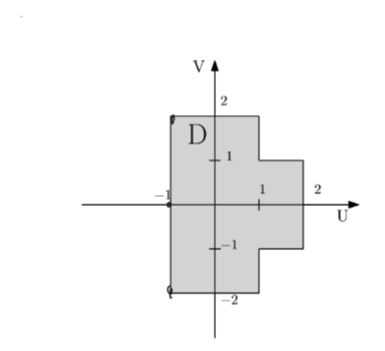
\includegraphics[width=0.45\textwidth]{dichte_aufgabe.png}
\end{center}
\begin{enumerate}[noitemsep,topsep=0pt,parsep=0pt,partopsep=0pt]  
  \item bestimme Konstnte $c$
  \item bestimme Randverteiungsfunktion von U und Randdichtefunktion $f_U(u)$.
  \item Sind $U$ und $V$ unabhängig?
\end{enumerate}
\begin{enumerate}[noitemsep,topsep=0pt,parsep=0pt,partopsep=0pt]  
  \item 
\begin{align*}
  D =  & \{(a, b) \in \mathbb{R}^2 : -1 \leq a \leq 1 \text{ and } -2 \leq b \leq 2\} \\
  \cup & \{(a, b) \in \mathbb{R}^2 : 1 \leq a \leq 2 \text{ and } -1 \leq b \leq 1\}  \\
       & f_{U,V}(u, v) =
  \begin{cases}
    1/10 & \text{if } (u, v) \in D \\
    0    & \text{otherwise}
  \end{cases}
\end{align*}
\item For $u < -1$, $F_U(u) = P(U \leq u) = 0$.
For $-1 \leq u \leq 1$, $F_U(u) = P(U \leq u) = $
\[
  \int_u^{-1} \int_{-2}^{2} \frac{1}{10} \mathbf{1}_D(u, v) \, dv \, ds = \frac{4(u + 1)}{10}
\]

For $1 \leq u \leq 2$, $F_U(u) = P(U \leq u) =$
\[
  \int_1^{-1} \int_{-2}^{2} \frac{1}{10} \mathbf{1}_D(u, v) \, dv \, ds + \int_u^1 \int_{-1}^{1} \frac{1}{10} \mathbf{1}_D(u, v) \, dv \, ds
\]
\[
  = \frac{8}{10} + \frac{2(u - 1)}{10}
\]

and $F_U(u) = 1$ for $u > 2$.

\[
  f_U(u) = \begin{cases}
    \frac{4}{10} & \text{if } -1 \leq u \leq 1 \\
    \frac{2}{10} & \text{if } 1 \leq u \leq 2  \\
    0            & \text{otherwise}
  \end{cases}
\]

\[
  f_V(v) = \int_{-\infty}^{\infty} f_{U,V}(u,v) \, du =
\]
\[
  \frac{1}{2}\left(2[v \in [-2,2]] + [v \in [-1,1]]\right)
\]

\item If U and V are independent, then for all u and v:

\[
  f_U(u) \cdot f_V(v) = f_{U,V}(u,v)
\]

However, we have \(f_{U,V}(2,2) = 0\) and \(f_U(2) \cdot f_V(2) = \frac{1}{5}
\cdot \frac{1}{5} \neq 0\).

Therefore, U and V are not independent.
\end{enumerate}
\end{tiny}
\BoxEnd{}
\subsection{Unabhängigkeit}
Die Zufallsvariablen $\zufallsvariablen$ heissen unabhängig, falls gilt
(äquivalent):
\begin{align*}
  F (x_1, \dots, x_n) = F_{X_1} (x_1) \cdot \hdots \cdot F_{X_n} (X_n) \\
  f (x_1, \dots, x_n) = f_{X_1} (x_1) \cdot \hdots \cdot f_{X_n} (X_n)
\end{align*}
für alle $x_1, \dots, x_n$.
\subsection{Bedingte Verteilungen}
Es gilt:
\begin{align*}
  f_{X_1 \; | \; X_2} (x_1 \; | \; x_2) & = \frac{f_{X_1,  X_2} (x_1,  x_2)}{f_{X_2} (x_2)}              \\
  \cond{Y > t}{Y < a}                   & = \frac{P[t < Y < a]}{P[Y < a]}                                \\
  E[X_1 \; | \; X_2]                    & = \int x_1 \cdot f_{x_1 \; | \; x_2} (x_1 \; | \; x_2) \; dx_1
\end{align*}
\subsection{Summen von Zufallsvariablen}
Sei $Z = X + Y$ eine Zufallsvariable mit:
\begin{align*}
  F_Z (z) & = P[Z \leq z] = P[X + Y \leq z]                                     \\
          & = \int_{-\infty}^\infty \int_{-\infty}^{z - x} f (x, y )\; dy \, dx \\
  f_Z (z) & = \int_{-\infty}^\infty f (z - y, y) \; dy
\end{align*}
\subsection{Transformationen}
Sei $X$ eine Zufallsvariable mit Verteilung und Dichte. Sei $g: \R \mapsto \R$
eine messbare Funktion. Betrachte nun $Y = g (X)$, wir suchen Verteilung und
Dichte von $Y$:
\begin{align*}
  F_Y (t) & = P[Y \leq t] = P[g (Y) \leq t] = \int_{A_g} f_X (s) \; ds \\
  A_g     & := \{s \in \R \; | \; g (s) \leq t\}
\end{align*}
Wobei man die Dichte durch ableiten der Verteilung erhält.
\subsection{Anwendung von Transformationen}
Sei $F$ eine stetige und streng monoton wachsende Verteilungsfunktion mit
Umkehrfunktion $F^{-1}$. Ist $X \sim \mathcal{U} (0, 1)$ und $Y = F^{-1} (X)$,
so hat $Y$ gerade die Verteilungsfunktion $F$:
\begin{align*}
  F_Y (t) & = P[Y \leq t] = P[F^{-1} (X) \leq t] \\
          & = P[X \leq F (t)] = F (t)
\end{align*}
Mit der Substitution
\begin{align*}
  \phi(X) & = Y                                              \\
  X       & = \phi^{-1}(y)                                   \\
  f_Y(y)  & = f_X(\phi^{-1}(y))|\text{det }J_{\phi^{-1}}(y)| \\
\end{align*}
\BoxStart{}
\subsection{Beispiel: Transformation}
Sei $X$ eine Zufallsvariable mit Dichte $f_X(x), x \in \R$ und sei $Y = e^X$. Was ist die Dichte $f_Y(y), y > 0$ der Zufallsvariable $Y$?
\begin{align*}
  Y             & = e^X                          \\
  X             & = \ln Y                        \\
  \frac{dx}{dy} & = \frac{1}{y}                  \\
  f_Y(y)        & = f_X(\ln y) \cdot \frac{1}{y} \\
\end{align*}

\BoxEnd{}
